%!TEX program = xelatex
% Note: this template must be compiled with XeLaTeX rather than PDFLaTeX
% due to the custom fonts used. The line above should ensure this happens
% automatically, but if it doesn't, your LaTeX editor should have a simple toggle
% to switch to using XeLaTeX.

\documentclass[
	aspectratio=169, % Uncomment to use an aspect ratio of 16:9 (160 mm by 90 mm)
	%aspectratio=43, % Uncomment to use an aspect ratio of 4:3 (128mm by 96mm)
	t, % Top align all slide content by default
	onlytextwidth, % Typeset content in columns at text width
	10pt, % Default font size, use 10pt for the 16:9 aspect ratio and 8pt for the 4:3 aspect ratio
]{beamer}


\usepackage{../../ImperialTheme/beamer/beamerthemeImperial} % Use the Imperial theme

\def\imagefolder{../../ImperialTheme/beamer/Images}



\title{Flat domain} % Presentation title to appear on the title slide and left footers

\subtitle{} % Presentation subtitle to appear on the title slide

\author{Víctor Ballester} % Author name(s) to appear on the title slide

\date{\today} % Presentation date to appear on the title slide and right footers

\begin{document}

\begingroup
\setbeamercolor{background canvas}{bg=ICLBlue} % Slide background color
\setbeamercolor{title page title}{fg=white} % Title text color
\setbeamercolor{title page subtitle}{fg=white} % Subtitle text color
\setbeamercolor{author}{fg=white} % Author(s) text color
\setbeamercolor{date}{fg=white} % Date text color
\setbeamertemplate{title page}[logo]{\imagefolder/ICL_Logo_White.pdf} % Imperial logo color, use 'ICL_Logo_White.pdf' for white and 'ICL_Logo_Blue.pdf' for blue
\frame[plain, s]{\titlepage} % Output the title page with no footer ('plain') and vertically distributed text ('s')
\endgroup

\begin{frame}
	\frametitle{Domain}
	
	\begin{itemize}
		\item Flat domain. I ran the baseflow till numerical steady state (I could set large $dt$).
		\item At the end I am using a full (small in height) BL of quads for the mesh.
		\item Previous length (upstream + gap + downstream): $L=(50 + 16.25 + 150)\delta^*= 216.25\delta^*$.
		\item New length: $650\delta^*$.
	\end{itemize}
	
	
        
\end{frame}
\begin{frame}
	\frametitle{Most unstable mode}
	First two eigenvalues are real.

	{
	\centering
	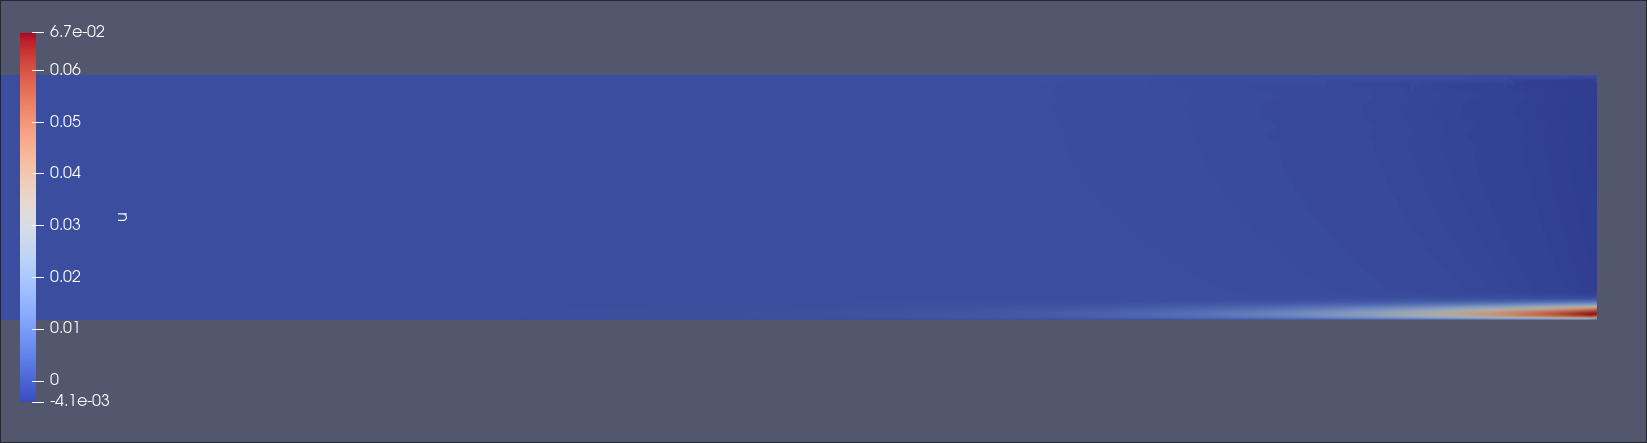
\includegraphics[width=\linewidth]{Images/ev.png}
	}

	There's an accumulation of energy at the outflow boudnary. I tried to increase the length of the domain to avoid this but it didn't work. Is it physical the mode?
	
\end{frame}
\end{document}
